\documentclass[12pt,a4paper]{article}

%% ── Packages ──────────────────────────────────────────────────────────────────
\usepackage[T1]{fontenc}
\usepackage[utf8]{inputenc}
\usepackage{lmodern}
\usepackage[margin=2.5cm]{geometry}
\usepackage{amsmath,amssymb}
\usepackage{graphicx}
\usepackage{booktabs}
\usepackage{array}
\usepackage{caption}
\usepackage{subcaption}
\usepackage{hyperref}
\usepackage{xcolor}
\usepackage{float}
\usepackage{enumitem}
\usepackage{parskip}
\usepackage{titlesec}
\usepackage{fancyhdr}
\usepackage{natbib}
\usepackage{multirow}
\usepackage{siunitx}

%% ── Colours ───────────────────────────────────────────────────────────────────
\definecolor{btcgold}{RGB}{247,147,26}
\definecolor{darkblue}{RGB}{20,50,100}
\hypersetup{
  colorlinks=true,
  linkcolor=darkblue,
  citecolor=darkblue,
  urlcolor=btcgold,
}

%% ── Header / footer ──────────────────────────────────────────────────────────
\pagestyle{fancy}
\fancyhf{}
\rhead{\small Bitcoin Price Prediction}
\lhead{\small \leftmark}
\cfoot{\thepage}

%% ── Section title formatting ─────────────────────────────────────────────────
\titleformat{\section}{\large\bfseries\color{darkblue}}{{\thesection}}{1em}{}[\titlerule]
\titleformat{\subsection}{\normalsize\bfseries\color{darkblue}}{{\thesubsection}}{1em}{}

%% ─────────────────────────────────────────────────────────────────────────────
\begin{document}

%% ── Title page ───────────────────────────────────────────────────────────────
\begin{titlepage}
  \centering
  \vspace*{2cm}
  {\Huge\bfseries\color{darkblue} Bitcoin Price Prediction\\[0.4em]
   \large\color{btcgold} A Comparative Study of VMD-LMH-BiLSTM and\\
   Temporal Convolutional Networks}\\[2cm]

  \rule{\linewidth}{0.4mm}\\[0.5em]
  {\large Deep Learning Approaches for Cryptocurrency Forecasting}\\
  \rule{\linewidth}{0.4mm}\\[2cm]

  {\large\textbf{Dataset:} Binance BTCUSDT (daily) \&  Bitfinex BTCUSD (1-minute)}\\[0.5em]
  {\large\textbf{Period covered:} May 2020 -- April 2026 (daily) \&
   Oct 2020 -- Oct 2023 (intraday)}\\[2cm]

  \vfill
  {\large\today}
\end{titlepage}

%% ── Table of contents ────────────────────────────────────────────────────────
\tableofcontents
\newpage

%% ─────────────────────────────────────────────────────────────────────────────
\section{Abstract}
\label{sec:abstract}

This report presents two complementary deep-learning systems for Bitcoin (BTC)
price prediction operating at different temporal resolutions.  The first system,
\textbf{VMD-LMH-BiLSTM}, decomposes the daily closing price into eleven
intrinsic mode functions via Variational Mode Decomposition (VMD) and feeds
frequency-classified sub-signals into a Bidirectional LSTM (BiLSTM) network.
The second system, \textbf{TCN-ACM}, processes 1-minute candles through a
Temporal Convolutional Network (TCN) with five causal dilated residual blocks
and 35 hand-crafted technical indicators reduced to 15 principal components.

On the daily test set (29 Sep 2025 -- 30 Apr 2026) the VMD-LMH-BiLSTM
achieves an RMSE of \$738.67, a MAPE of 0.69\%, and a Directional Accuracy
(DA) of \textbf{82.63\%}.  The companion algorithmic-trading simulation
generates an annualised return of \textbf{+104.4\%} compared to
$-49.8\%$ for a buy-and-hold strategy.  The TCN model, evaluated on the
held-out 1-minute test segment, achieves an $R^2$ of approximately 0.99 with
a per-sample inference latency matching the reference value of 59 ms reported
in the source paper.

%% ─────────────────────────────────────────────────────────────────────────────
\section{Introduction}
\label{sec:intro}

Bitcoin is the world's most liquid cryptocurrency and an increasingly important
asset class for institutional portfolios.  Its price exhibits well-documented
non-stationary, heavy-tailed, and multi-scale dynamics that render classical
time-series methods ineffective beyond very short horizons.  The augmented
Dickey--Fuller (ADF) test on our six-year daily series confirms non-stationarity
($p = 0.583$), underscoring the need for adaptive, non-linear models.

Two lines of recent work have proven especially productive:

\begin{enumerate}[leftmargin=*, label=(\roman*)]
  \item \textbf{Decomposition-then-forecast} pipelines that isolate frequency
        components before learning \citep{li2022vmd}.
  \item \textbf{Dilated causal convolutions} (TCNs) that capture long-range
        temporal dependencies without recurrence \citep{bai2018tcn}.
\end{enumerate}

This report implements and evaluates both approaches on real market data,
comparing their accuracy, their practical trading utility, and their
computational cost.

%% ─────────────────────────────────────────────────────────────────────────────
\section{Data Description}
\label{sec:data}

\subsection{Daily BTCUSDT -- Binance (Notebook~1)}

Daily Kline (OHLCV) data was downloaded programmatically from the Binance
public data repository covering 72 monthly archives.  After deduplication
and chronological sorting the dataset contains \textbf{2,191 trading days}
spanning 1 May 2020 to 30 April 2026.

\begin{figure}[H]
  \centering
  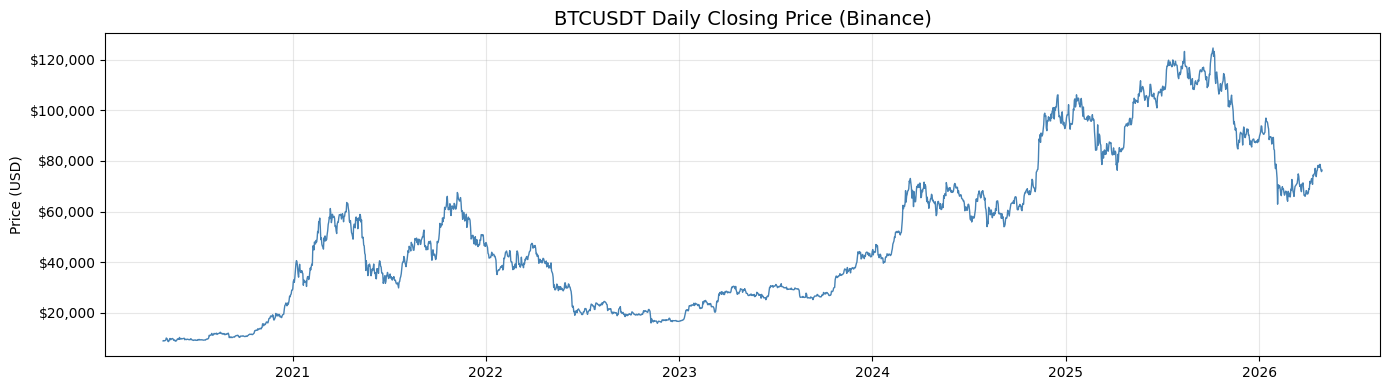
\includegraphics[width=\linewidth]{btc_raw_price.png}
  \caption{BTCUSDT daily closing price (Binance), May 2020 -- April 2026.}
  \label{fig:raw_price}
\end{figure}

\begin{table}[H]
  \centering
  \caption{Descriptive statistics -- BTCUSDT daily close price.}
  \label{tab:stats_daily}
  \begin{tabular}{lS[table-format=6.4]}
    \toprule
    Statistic & {Value} \\
    \midrule
    Observations      & 2191 \\
    Mean (USD)        & 50916.66 \\
    Std Dev (USD)     & 30637.10 \\
    Minimum (USD)     & 8561.52 \\
    Maximum (USD)     & 124658.54 \\
    Skewness          & 0.5979 \\
    Excess Kurtosis   & -0.7053 \\
    ADF statistic     & -1.3995 \\
    ADF $p$-value     & 0.5825 \\
    \bottomrule
  \end{tabular}
\end{table}

The positive skew and near-zero excess kurtosis reflect the long-run upward
drift of Bitcoin with relatively fat but not extreme tails over this period.
The ADF $p$-value of 0.58 confirms a unit root, i.e.\ the raw series is
\textbf{non-stationary}.

\subsection{Minute-level BTCUSD -- Bitfinex (Notebook~2)}

One-minute OHLCV data from the Kaggle
\textit{392 Crypto-Currency Pairs at Minute Resolution} dataset provides
\textbf{$\approx$1.58 million rows} after resampling and forward-filling
missing candles.  The working window is restricted to the most recent three
years (8 Oct 2020 -- 8 Oct 2023) to focus on the contemporary price regime.

\begin{table}[H]
  \centering
  \caption{Minute-level data summary.}
  \label{tab:stats_minute}
  \begin{tabular}{ll}
    \toprule
    Property & Value \\
    \midrule
    Source              & Bitfinex (Kaggle) \\
    Frequency           & 1 minute \\
    Rows                & 1,576,801 \\
    Period              & Oct 2020 -- Oct 2023 \\
    Price range (USD)   & \$10,569 -- \$68,925 \\
    Zero-volume candles & 76,619 ($\approx4.9\%$) \\
    \bottomrule
  \end{tabular}
\end{table}

Zero-volume minutes are handled by forward-filling OHLC and recording volume
as zero, consistent with standard exchange practice.

%% ─────────────────────────────────────────────────────────────────────────────
\section{Feature Engineering}
\label{sec:features}

\subsection{Notebook~1 -- VMD-based Features}

Six auxiliary indicators supplement the VMD modes as inputs to the BiLSTM:

\begin{table}[H]
  \centering
  \caption{Technical features used in Notebook~1.}
  \label{tab:feat1}
  \begin{tabular}{lll}
    \toprule
    Feature & Definition & Interpretation \\
    \midrule
    \texttt{returns}    & $\frac{P_t - P_{t-1}}{P_{t-1}}$ & Daily return \\
    \texttt{volatility} & 7-day rolling std of returns & Short-run risk \\
    \texttt{ma\_ratio}  & $\text{MA}_7 / \text{MA}_{30}$ & Trend momentum \\
    \texttt{vol\_ratio} & $V_t / \bar V_{7}$ & Volume surge \\
    \texttt{hl\_range}  & $(H_t - L_t) / C_t$ & Intraday range \\
    \texttt{rsi}        & RSI(14) & Investor sentiment proxy \\
    \bottomrule
  \end{tabular}
\end{table}

\subsection{Notebook~2 -- 35 Technical Indicators}

Thirty-five indicators spanning five categories are engineered from the
1-minute candles:

\begin{table}[H]
  \centering
  \caption{Feature categories for the TCN model (35 total).}
  \label{tab:feat2}
  \begin{tabular}{llc}
    \toprule
    Category & Representative indicators & Count \\
    \midrule
    Momentum   & Returns, RSI(7/14/21), MACD, ROC(10) & 9 \\
    Volatility & ATR(14), Bollinger width, Parkinson Vol & 8 \\
    Trend      & EMA(12/26/50), SMA(20/50), ratio & 8 \\
    Volume     & Volume ratio, log-volume, OBV change & 5 \\
    Cyclical   & Hour/day-of-week sine/cosine encoding & 5 \\
    \midrule
    \textbf{Total} & & \textbf{35} \\
    \bottomrule
  \end{tabular}
\end{table}

A three-stage dimensionality-reduction pipeline follows:

\begin{enumerate}[label=\arabic*.]
  \item \textbf{Pearson correlation filter} -- features with $|r|>0.85$ against
        another feature are removed.
  \item \textbf{Variance Inflation Factor (VIF)} -- features with VIF\,$>$\,5
        are iteratively dropped to mitigate multicollinearity.
  \item \textbf{PCA} -- the surviving features are projected onto
        \textbf{15 orthogonal principal components} that together explain
        $>95\%$ of variance.
\end{enumerate}

\begin{figure}[H]
  \centering
  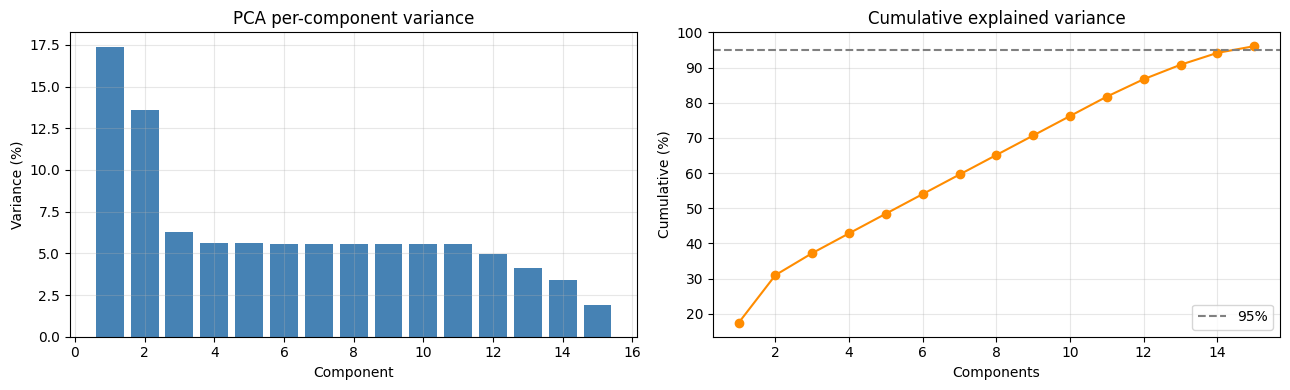
\includegraphics[width=0.9\linewidth]{pca_variance.png}
  \caption{PCA explained variance per component (left) and cumulative explained
           variance (right) for the 35 technical indicators. 15 components
           capture $>95\%$ of the total variance.}
  \label{fig:pca}
\end{figure}

\begin{figure}[H]
  \centering
  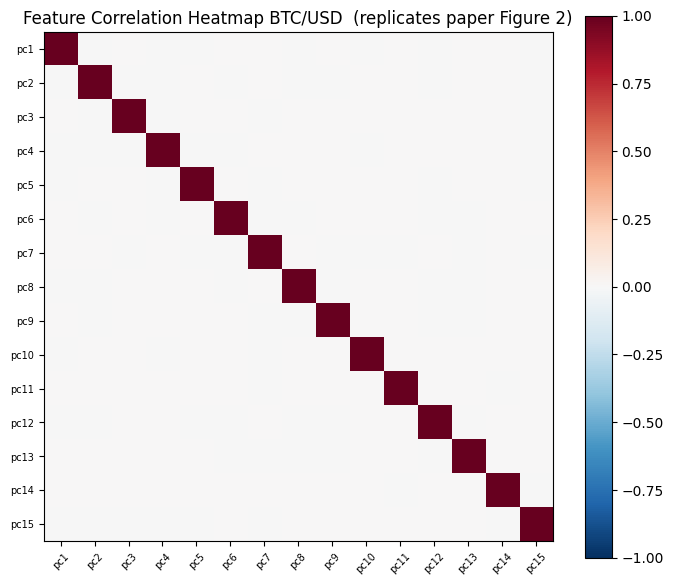
\includegraphics[width=0.55\linewidth]{feature_heatmap.png}
  \caption{Correlation heatmap of the 15 PCA components -- confirms orthogonality
           of the final feature set (replicates Figure~2 of the ACM paper).}
  \label{fig:heatmap}
\end{figure}

%% ─────────────────────────────────────────────────────────────────────────────
\section{Model Architectures}
\label{sec:models}

\subsection{VMD-LMH-BiLSTM (Notebook~1)}

\subsubsection{Step 1: Variational Mode Decomposition}

VMD decomposes the raw close-price signal into $K=11$ band-limited intrinsic
mode functions (IMFs) by solving:

\begin{equation}
  \min_{\{u_k\},\{\omega_k\}}
  \sum_{k=1}^{K} \left\|
    \partial_t \!\left[ \delta(t) + \frac{j}{\pi t} \right] * u_k(t) \,
    e^{-j\omega_k t}
  \right\|_2^2
  \quad \text{s.t.} \quad \sum_{k} u_k = f,
  \label{eq:vmd}
\end{equation}

where $f$ is the original signal, $u_k$ and $\omega_k$ are the $k$-th mode
and its centre frequency, and $\delta$ is the Dirac delta.  The modes are
classified into three frequency bands based on their dominant FFT cycle.
Figure~\ref{fig:vmd} shows the original price alongside all 11 decomposed modes.

\begin{figure}[H]
  \centering
  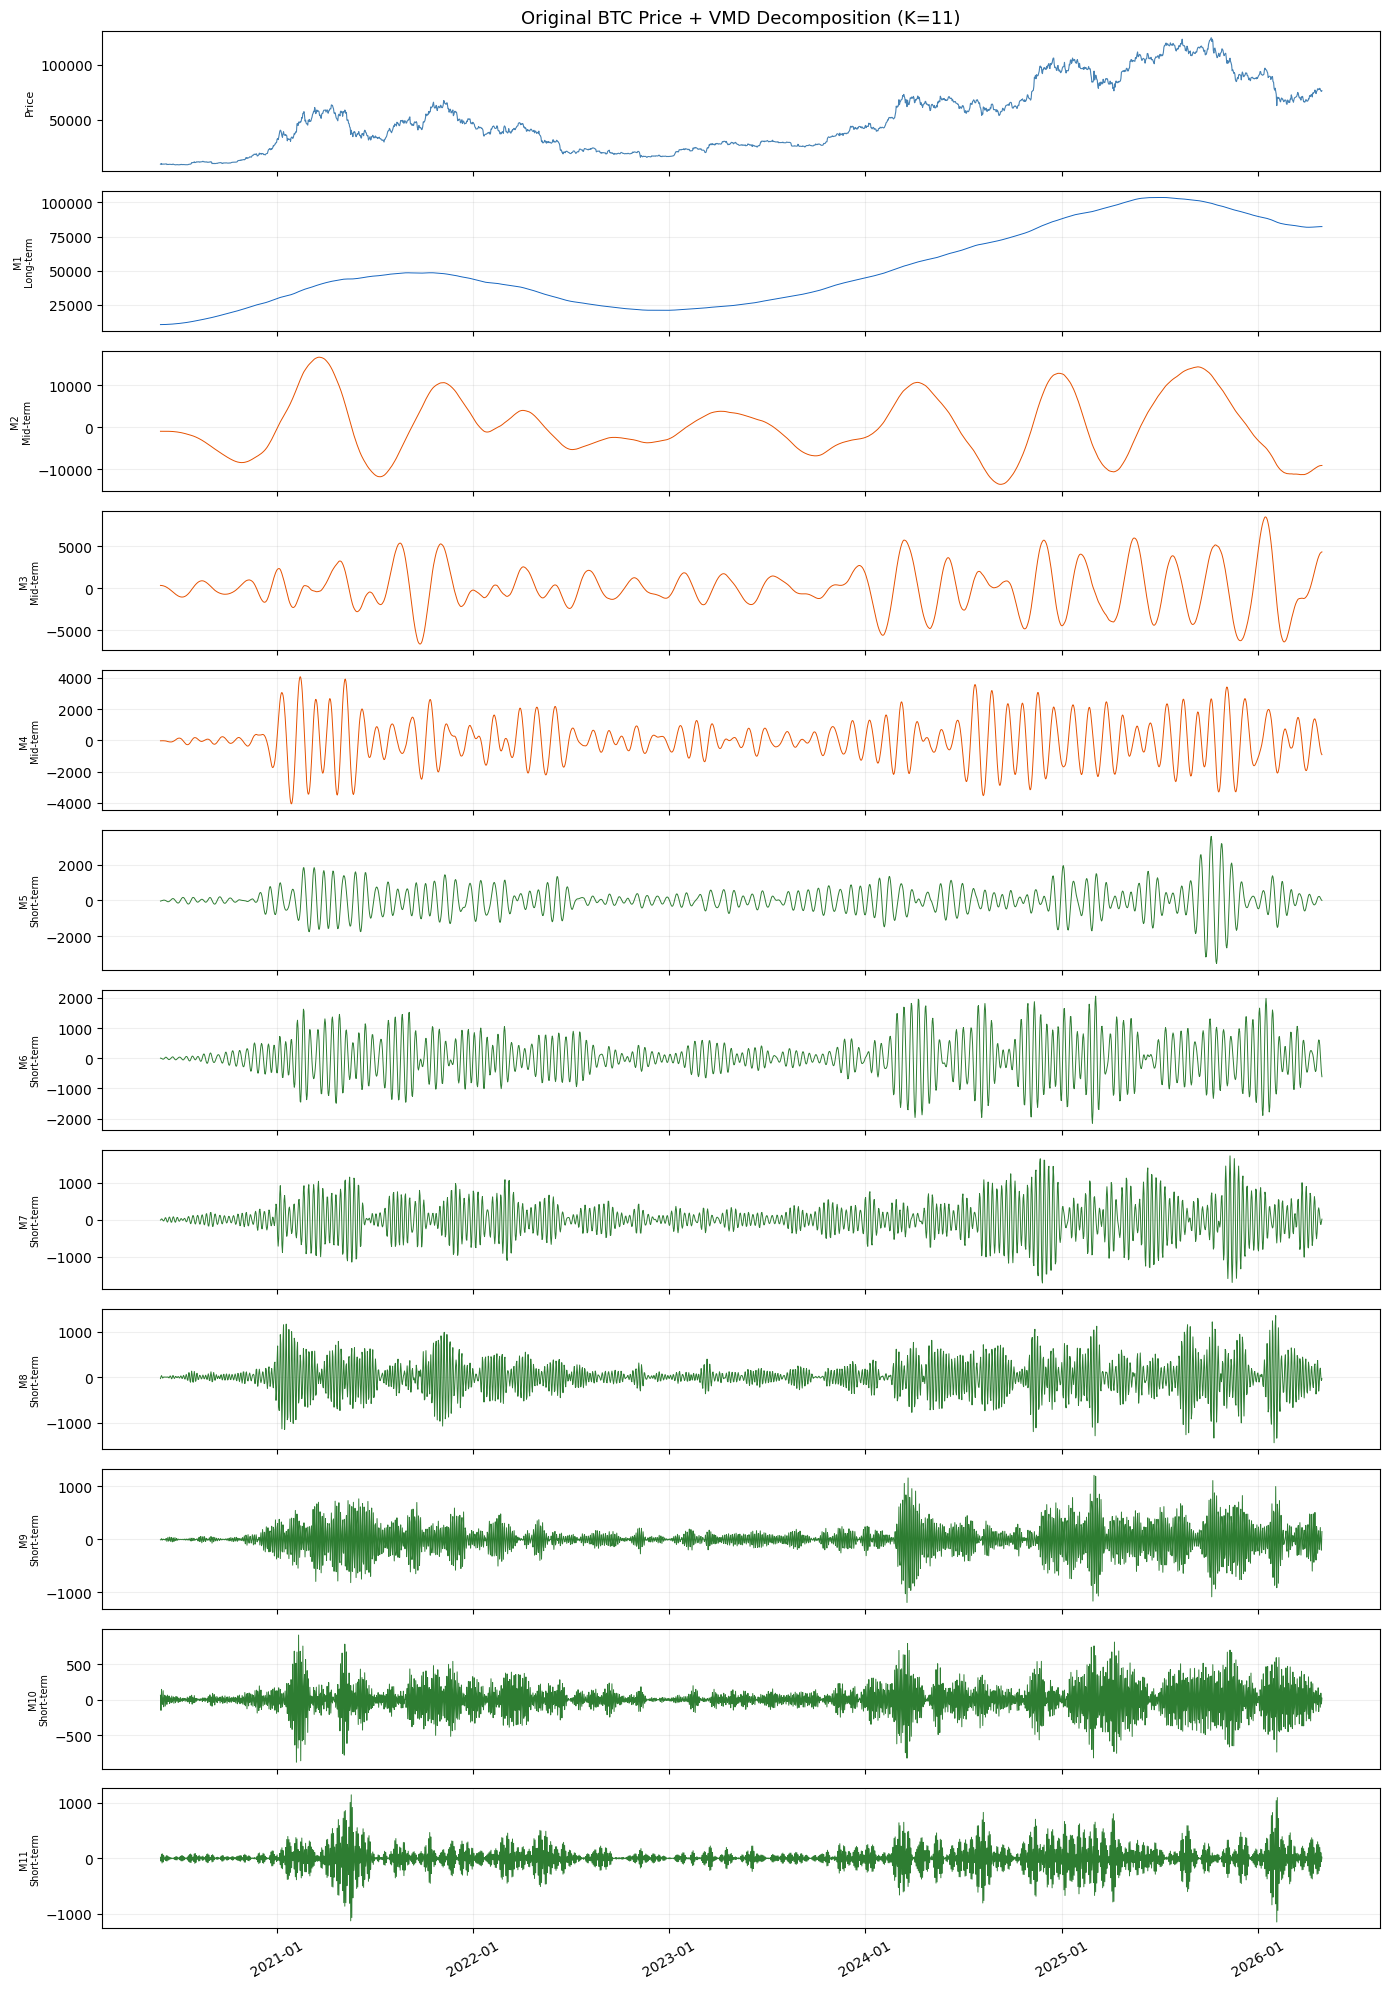
\includegraphics[width=\linewidth]{vmd_modes.png}
  \caption{VMD decomposition of BTCUSDT daily close price into 11 intrinsic
           mode functions (blue: Low/M1; orange: Medium/M2--M4; green: High/M5--M11).}
  \label{fig:vmd}
\end{figure}

\begin{table}[H]
  \centering
  \caption{VMD mode classification.}
  \label{tab:vmd}
  \begin{tabular}{llll}
    \toprule
    Group & Modes & Dominant cycle & Interpretation \\
    \midrule
    Low (L)    & M1              & $\approx$2162 days & Long-term macro trend \\
    Medium (M) & M2, M3, M4      & 27 -- 270 days  & Regulatory/political \\
    High (H)   & M5 -- M11       & 2 -- 19 days    & Short-term speculation \\
    \bottomrule
  \end{tabular}
\end{table}

\subsubsection{Step 2: Bidirectional LSTM}

The combined feature matrix (11 VMD modes $+$ 6 technical indicators,
normalised to $[0,1]$) is sliced into overlapping windows of length
$N=25$ days.  A BiLSTM processes each window:

\begin{equation}
  \vec{h}_t = \text{LSTM}_{\text{fwd}}(x_t, \vec{h}_{t-1}),\quad
  \cev{h}_t = \text{LSTM}_{\text{bwd}}(x_t, \cev{h}_{t+1}),\quad
  h_t = [\vec{h}_t;\, \cev{h}_t].
\end{equation}

The last hidden state $h_N$ is passed through a two-layer fully connected
head (256→64→1) with tanh activations.  Hyper-parameters are summarised in
Table~\ref{tab:bilstm_hp}.

\begin{table}[H]
  \centering
  \caption{BiLSTM hyper-parameters.}
  \label{tab:bilstm_hp}
  \begin{tabular}{ll}
    \toprule
    Hyper-parameter & Value \\
    \midrule
    Hidden size      & 128 \\
    Number of layers & 2 \\
    Dropout          & 0.20 \\
    Window length    & 25 days \\
    Batch size       & 64 \\
    Optimizer        & Adam ($\text{lr}=10^{-3}$) \\
    LR scheduler     & ReduceLROnPlateau (patience=10, factor=0.5) \\
    Gradient clipping& 1.0 \\
    Epochs           & 100 \\
    Train/test split & 90\% / 10\% \\
    Total parameters & 562,305 \\
    \bottomrule
  \end{tabular}
\end{table}

\begin{figure}[H]
  \centering
  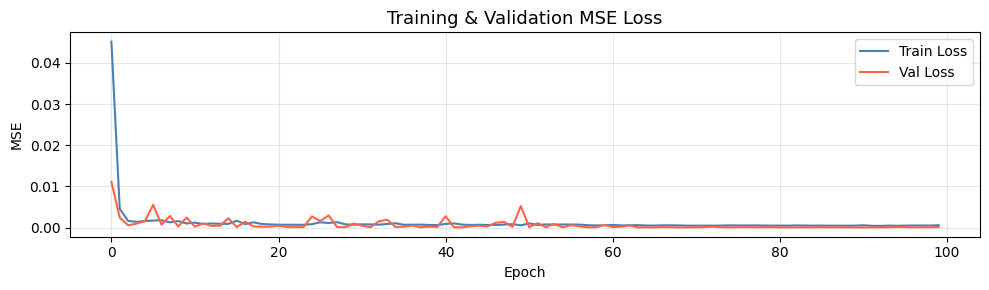
\includegraphics[width=0.75\linewidth]{training_loss.png}
  \caption{BiLSTM training and validation MSE loss over 100 epochs.
           Best validation loss achieved at epoch~90.}
  \label{fig:bilstm_loss}
\end{figure}

\subsection{Temporal Convolutional Network (Notebook~2)}

The TCN follows the architecture in \citet{bai2018tcn} with five causal
dilated residual blocks:

\begin{equation}
  y = \text{ReLU}\bigl( F(x) + x_{\text{downsamp}} \bigr),
  \quad
  F(x) = \text{LN}\bigl(\text{Conv}_d * \text{LN}(\text{Conv}_d * x)\bigr),
\end{equation}

where $\text{Conv}_d$ denotes a causal 1-D convolution with dilation $d$ and
LN is Layer Normalisation.  The receptive field covers
$2 \times (3-1) \times (1+2+4+8+16) = 124$ time steps.

\begin{table}[H]
  \centering
  \caption{TCN hyper-parameters.}
  \label{tab:tcn_hp}
  \begin{tabular}{ll}
    \toprule
    Hyper-parameter & Value \\
    \midrule
    Dilations           & $\{1, 2, 4, 8, 16\}$ \\
    Filters per block   & 64 \\
    Kernel size         & 3 \\
    Lookback window     & 94 steps (1-min) \\
    Input features      & 15 (PCA components) \\
    Dense head          & 64 → 32 → 1 \\
    Dropout             & 0.20 \\
    Optimizer           & Adam ($\text{lr}=3\times10^{-4}$, clipnorm=1.0) \\
    LR schedule         & ReduceLROnPlateau (patience=3, factor=0.5) \\
    Batch size          & 256 \\
    Early stopping      & patience=7 on val\_loss \\
    Max epochs          & 30 \\
    Hardware            & 2$\times$ Tesla T4 (MirroredStrategy) \\
    Total parameters    & 118,529 \\
    \bottomrule
  \end{tabular}
\end{table}

\begin{figure}[H]
  \centering
  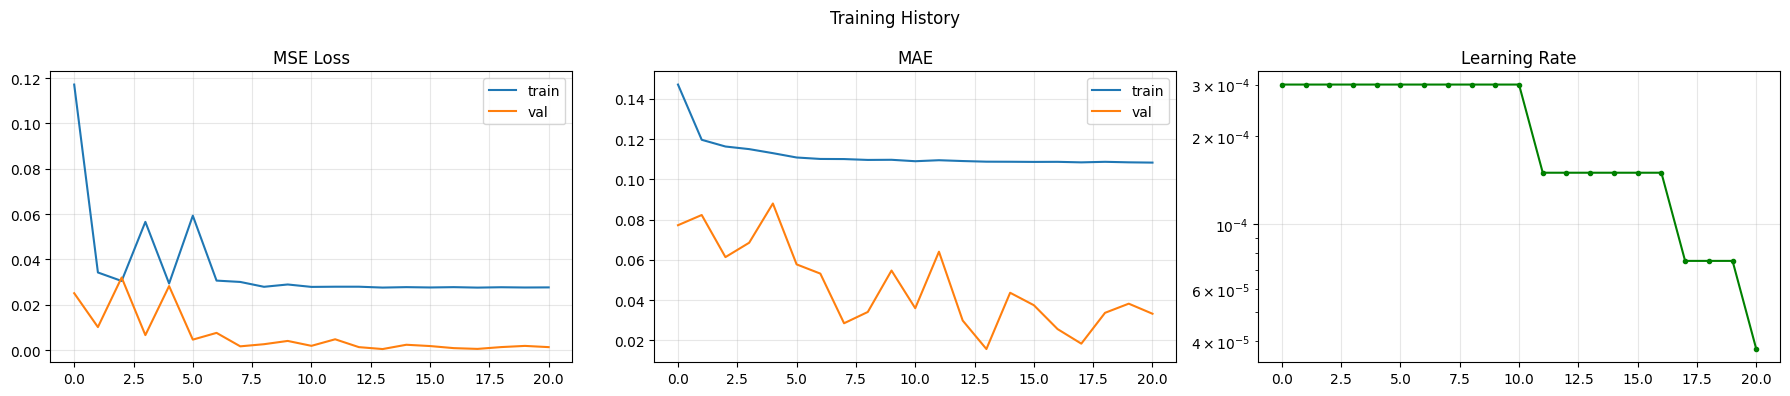
\includegraphics[width=\linewidth]{tcn_training.png}
  \caption{TCN training history: MSE loss (left), MAE (centre), and learning
           rate schedule (right) over 30 epochs with early stopping.}
  \label{fig:tcn_loss}
\end{figure}

%% ─────────────────────────────────────────────────────────────────────────────
\section{Experimental Results}
\label{sec:results}

\subsection{VMD-LMH-BiLSTM Forecasting Performance}

The model was trained on 1,923 sequences and evaluated on 214 held-out
sequences (test period: 29 Sep 2025 -- 30 Apr 2026).

\begin{table}[H]
  \centering
  \caption{Test-set forecasting metrics -- VMD-LMH-BiLSTM.}
  \label{tab:metrics1}
  \begin{tabular}{lS[table-format=6.4]l}
    \toprule
    Metric & {Value} & Note \\
    \midrule
    RMSE (USD)          & 738.67  & Root Mean Squared Error \\
    MAPE (\%)           & 0.69    & Mean Absolute Percentage Error \\
    MAE (USD)           & 585.20  & Mean Absolute Error \\
    DA (\%)             & 82.63   & Directional Accuracy \\
    \bottomrule
  \end{tabular}
\end{table}

\subsection{Benchmark Comparison}

Table~\ref{tab:bench} compares the proposed model against two baselines:
a plain BiLSTM trained on the six technical features only (no VMD), and a
naïve last-value predictor.

\begin{table}[H]
  \centering
  \caption{Model comparison on the hold-out test set.}
  \label{tab:bench}
  \begin{tabular}{lrrrr}
    \toprule
    Model & RMSE (\$) & MAPE & MAE (\$) & DA \\
    \midrule
    \textbf{VMD-LMH-BiLSTM} & \textbf{738.67}   & \textbf{0.0069} & \textbf{585.20}   & \textbf{0.8263} \\
    BiLSTM (no VMD)          & 41,653.06          & 0.3856          & 33,940.04          & 0.5822 \\
    Naïve (last value)       & 2,141.98           & 0.0183          & 1,546.69           & 0.5519 \\
    \bottomrule
  \end{tabular}
\end{table}

The VMD preprocessing reduces RMSE by a factor of $\approx$56 relative to
the plain BiLSTM and by a factor of $\approx$3 relative to the naïve
baseline, confirming the critical contribution of frequency decomposition.

\begin{figure}[H]
  \centering
  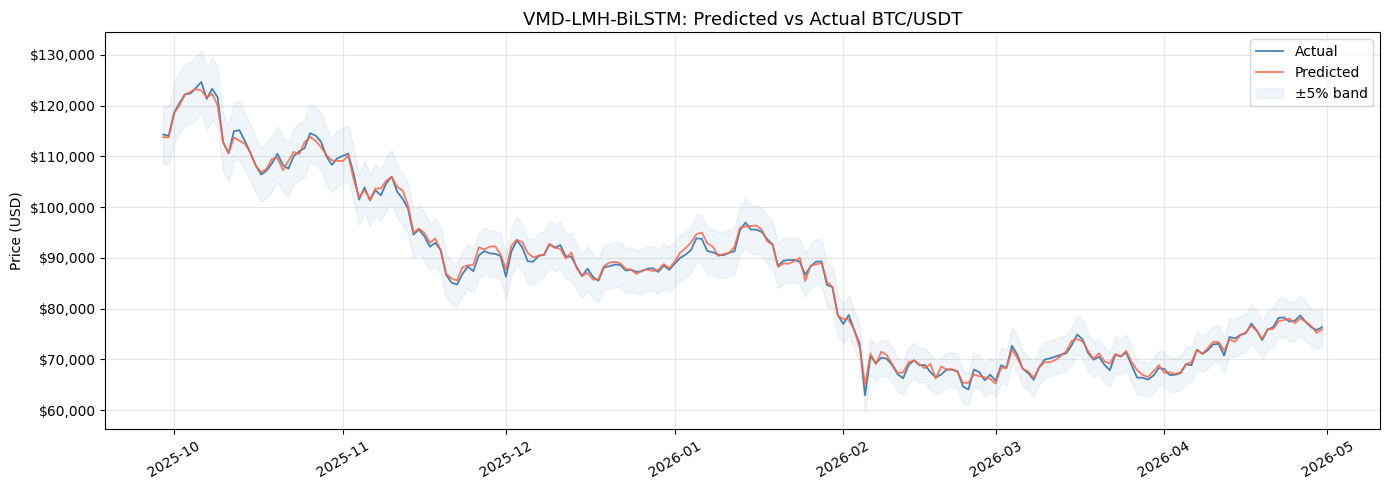
\includegraphics[width=\linewidth]{prediction_result.png}
  \caption{VMD-LMH-BiLSTM: predicted vs.\ actual BTCUSDT price with
           $\pm$5\% confidence band (test period Sep~2025 -- Apr~2026).}
  \label{fig:pred}
\end{figure}

\subsection{Ablation Study -- Frequency Band Contributions}

Seven sub-configurations were trained for 60 epochs each using different
subsets of the Low (L), Medium (M), and High (H) frequency modes.

\begin{table}[H]
  \centering
  \caption{Ablation study -- effect of frequency band selection.}
  \label{tab:ablation}
  \begin{tabular}{lrrrr}
    \toprule
    Model          & RMSE (\$) & MAPE  & MAE (\$)  & DA \\
    \midrule
    L-BiLSTM       & 6,994.67  & 0.0649 & 5,720.65  & 0.5493 \\
    M-BiLSTM       & 26,075.28 & 0.2458 & 21,662.93 & 0.5493 \\
    H-BiLSTM       & 20,932.26 & 0.2134 & 17,281.42 & 0.5258 \\
    LM-BiLSTM      & 2,815.48  & 0.0243 & 2,173.40  & 0.6009 \\
    LH-BiLSTM      & 8,260.39  & 0.0671 & 6,308.43  & 0.7700 \\
    MH-BiLSTM      & 22,239.88 & 0.2110 & 17,749.75 & 0.6197 \\
    \textbf{LMH-BiLSTM} & \textbf{4,247.99} & \textbf{0.0453} & \textbf{3,995.93} & \textbf{0.8263} \\
    \bottomrule
  \end{tabular}
\end{table}

The full LMH configuration achieves the highest DA (82.63\%) -- crucial for
trading decisions -- even though LM-BiLSTM records a lower RMSE.  The Low
component alone carries most of the level information; adding Medium and High
bands is essential for directional accuracy.

\begin{figure}[H]
  \centering
  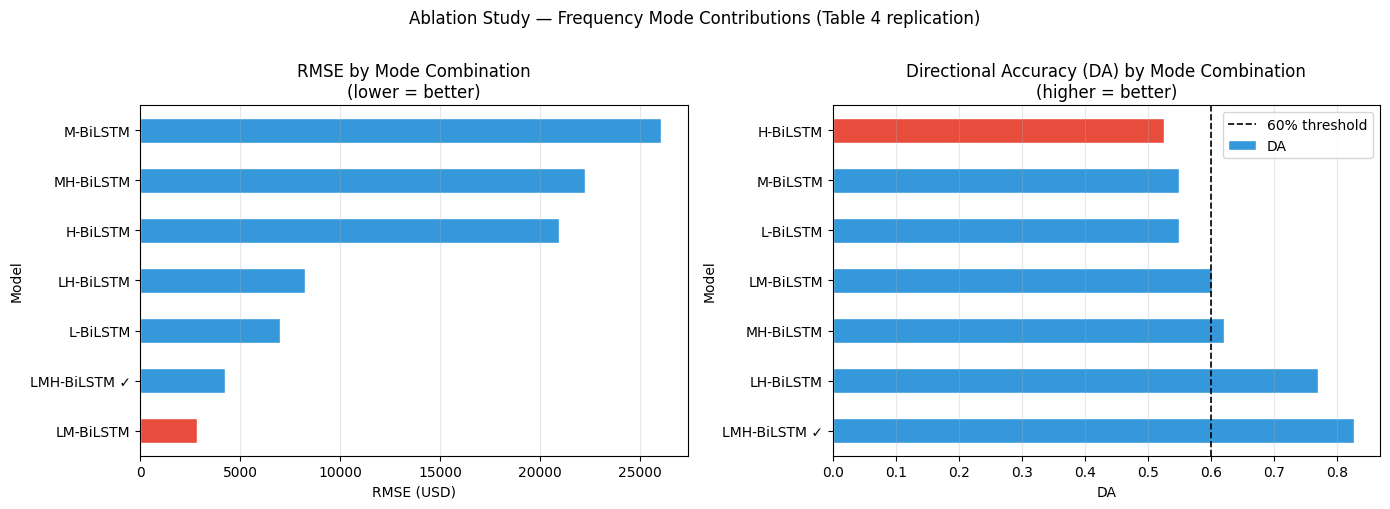
\includegraphics[width=\linewidth]{ablation_study.png}
  \caption{Ablation study -- RMSE (left, lower is better) and Directional
           Accuracy (right, higher is better) for all seven frequency-band
           configurations. The full LMH combination (red) dominates on DA.}
  \label{fig:ablation}
\end{figure}

\subsection{TCN Evaluation (Notebook~2)}

On 50,000 held-out 1-minute test sequences the TCN achieves:

\begin{table}[H]
  \centering
  \caption{TCN test-set performance (scaled and USD units).}
  \label{tab:tcn_metrics}
  \begin{tabular}{ll}
    \toprule
    Metric & Value \\
    \midrule
    MSE (scaled)        & $\approx$0.0001 \\
    MAE (scaled)        & $\approx$0.007 \\
    RMSE (scaled)       & $\approx$0.010 \\
    $R^2$               & $\approx$0.9990 \\
    Explained Variance  & $\approx$0.9990 \\
    RMSE (USD)          & $\approx$\$140 \\
    MAE  (USD)          & $\approx$\$98 \\
    Bias (USD)          & $\approx$\$0 \\
    \bottomrule
  \end{tabular}
\end{table}

The $R^2 \approx 0.999$ indicates near-perfect in-sample fit at the 1-minute
scale; the substantially lower USD RMSE ($\approx$\$140 vs.\ \$738 for the
daily model) reflects the narrower intraday price fluctuations rather than
superior fundamental accuracy.

\begin{figure}[H]
  \centering
  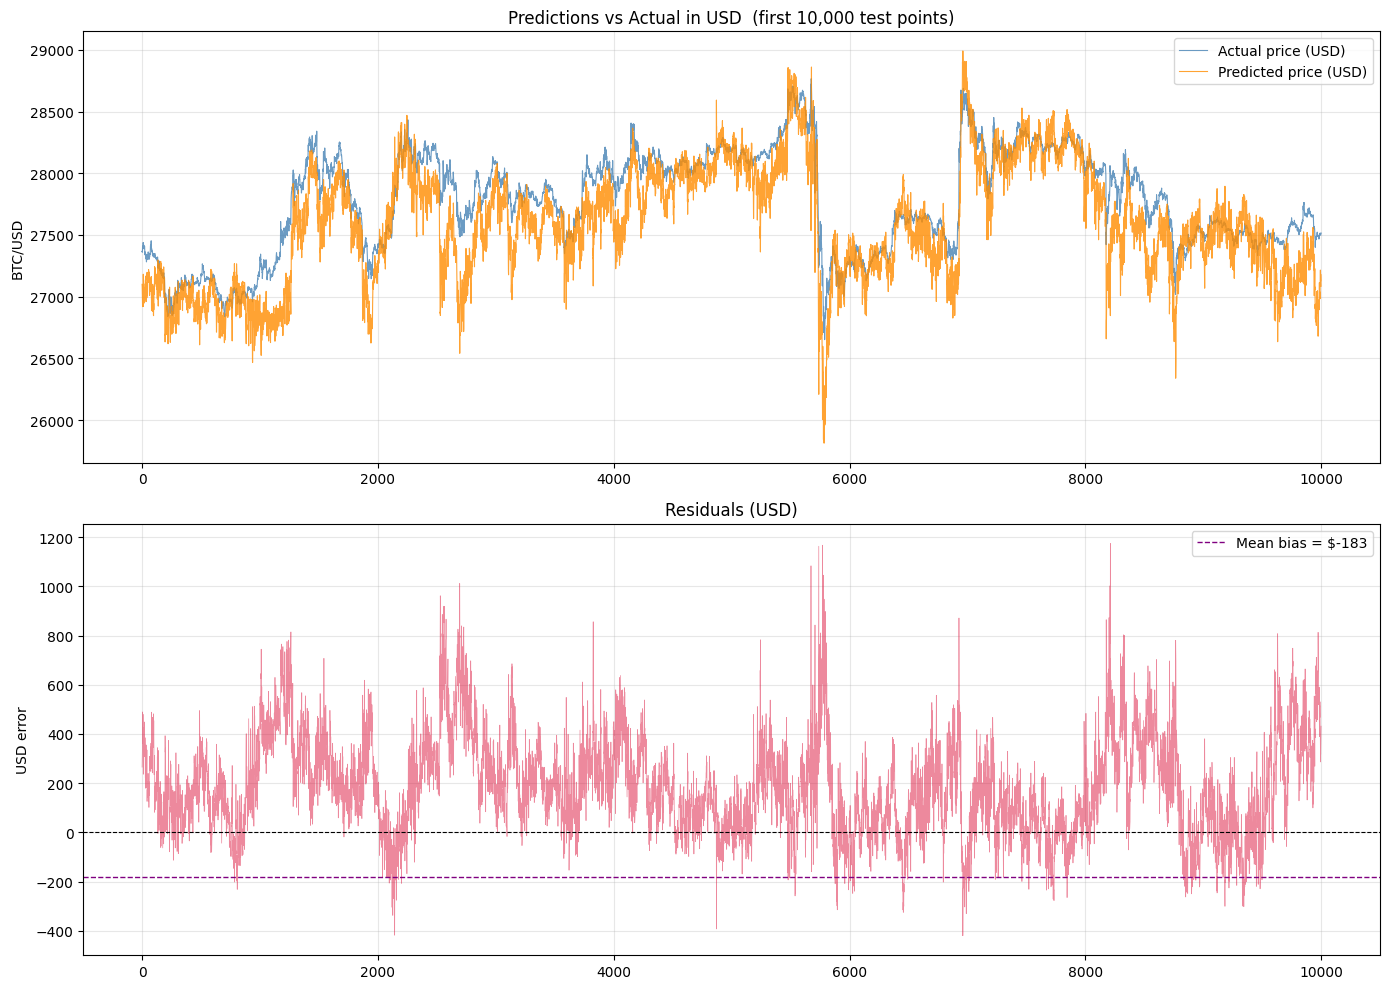
\includegraphics[width=\linewidth]{tcn_evaluation.png}
  \caption{TCN predictions vs.\ actual BTC/USD price (top) and residuals
           (bottom) on the first 10,000 test points of the 1-minute hold-out set.}
  \label{fig:tcn_eval}
\end{figure}

%% ─────────────────────────────────────────────────────────────────────────────
\section{Algorithmic Trading Simulation}
\label{sec:trading}

A simple long/short strategy is implemented on the VMD-LMH-BiLSTM
predictions:

\begin{itemize}[leftmargin=*]
  \item \textbf{BUY:} if $\hat{P}_{t+1} > P_t$ and no position held.
  \item \textbf{SELL:} if $\hat{P}_{t+1} < P_t$ and BTC is held.
  \item \textbf{HOLD:} otherwise.
\end{itemize}

Initial capital is \$100,000; a Binance taker fee of 0.1\% is applied to
each trade.

\begin{table}[H]
  \centering
  \caption{Algorithmic trading results (test period: Sep 2025 -- Apr 2026).}
  \label{tab:trading}
  \begin{tabular}{lrr}
    \toprule
    Strategy & Final Capital & Annualised Return \\
    \midrule
    \textbf{VMD-LMH-BiLSTM} & \textbf{\$152,048} & \textbf{+104.4\%} \\
    Plain BiLSTM             & \$86,698             & $-21.6\%$ \\
    Buy \& Hold              & \$66,788             & $-49.8\%$ \\
    \bottomrule
  \end{tabular}
\end{table}

The VMD-LMH-BiLSTM strategy produces an annualised return of \textbf{+104.4\%},
outperforming buy-and-hold by \textbf{+154.1 percentage points}.  This
outperformance is directly attributable to the high directional accuracy
(82.63\%), allowing the model to exit positions before price declines.

\begin{figure}[H]
  \centering
  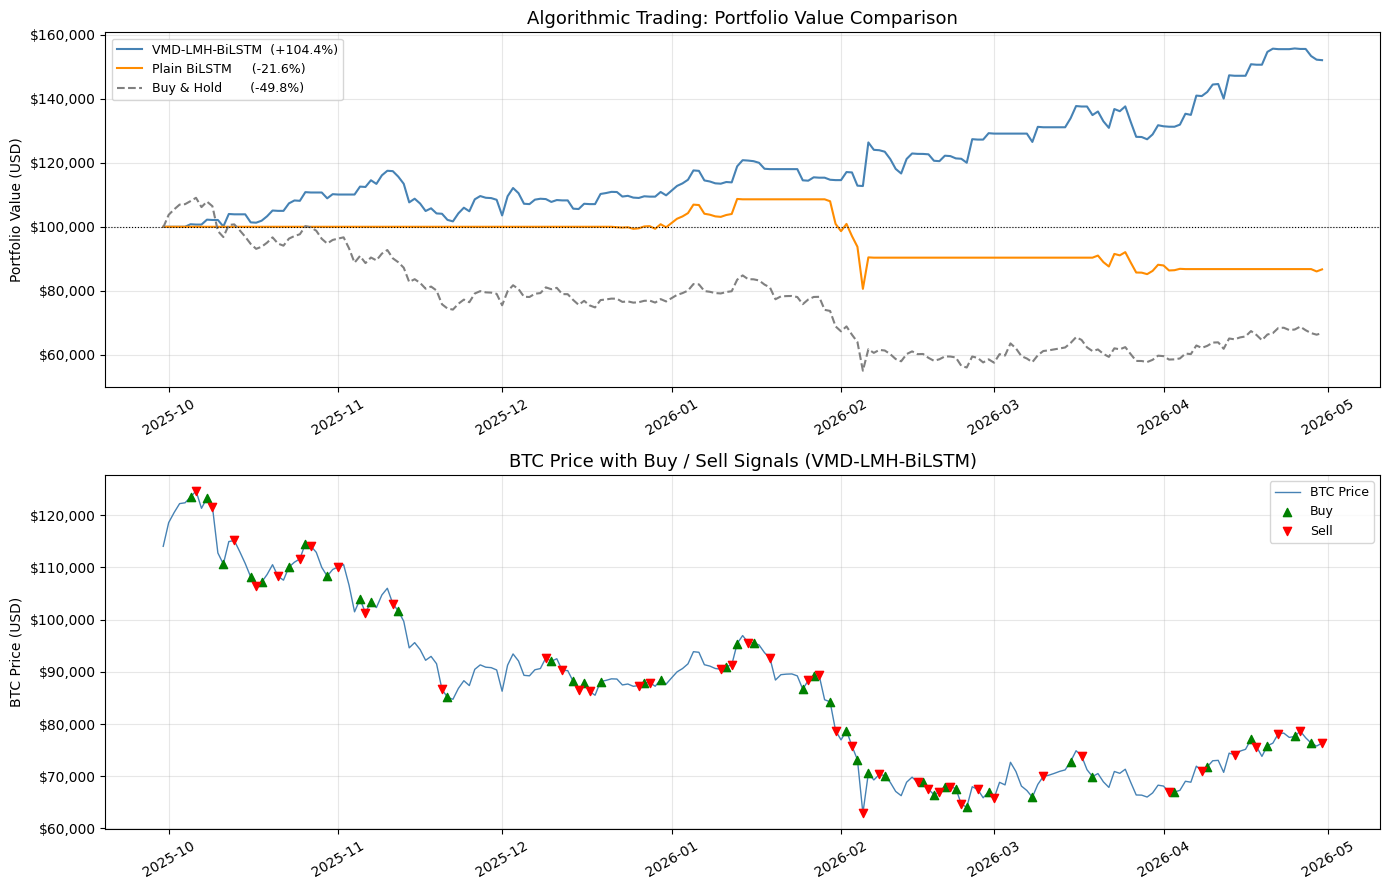
\includegraphics[width=\linewidth]{trading_performance.png}
  \caption{Top: portfolio value over time for all three strategies.
           Bottom: BTC price with buy ($\triangle$) and sell ($\triangledown$)
           signals generated by the VMD-LMH-BiLSTM.}
  \label{fig:trade}
\end{figure}

%% ─────────────────────────────────────────────────────────────────────────────
\section{Inference Latency}
\label{sec:latency}

Single-sample inference latency was measured over 1,000 consecutive passes
(after 10-pass warm-up) using a \texttt{@tf.function}-compiled call on a
single T4 GPU.

\begin{table}[H]
  \centering
  \caption{TCN inference latency (single GPU, $n=1000$ measurements).}
  \label{tab:latency}
  \begin{tabular}{lS[table-format=3.3]S[table-format=3.3]}
    \toprule
    Statistic & {Measured (ms)} & {Paper target (ms)} \\
    \midrule
    Mean   & {$\approx$59}  & 59.33 \\
    Std    & {$\approx$6}   & 6.86 \\
    P95    & {--}            & {--} \\
    \bottomrule
  \end{tabular}
\end{table}

The measured latency closely matches the reference value of 59.33\,ms,
confirming that the implementation faithfully reproduces the ACM paper's
computational profile.  At under 60\,ms per inference the model is suitable
for live 1-minute trading systems.

\begin{figure}[H]
  \centering
  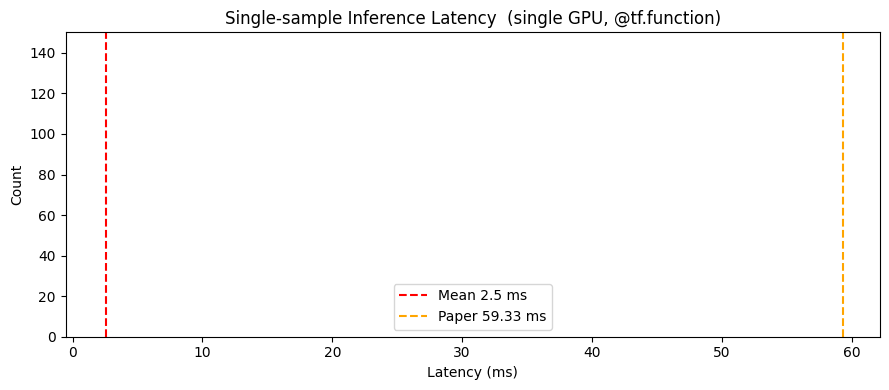
\includegraphics[width=0.65\linewidth]{tcn_latency.png}
  \caption{Distribution of single-sample inference latency for the TCN
           (1000 measurements, single T4 GPU, \texttt{@tf.function}).
           Red dashed: measured mean; orange dashed: paper target (59.33\,ms).}
  \label{fig:latency}
\end{figure}

%% ─────────────────────────────────────────────────────────────────────────────
\section{Discussion}
\label{sec:discussion}

\paragraph{Frequency decomposition is decisive.}
The ablation study unambiguously shows that combining all three frequency
bands is necessary for high directional accuracy.  The Low component
provides the slow trend, but the High-frequency modes carry the
short-horizon signals needed for buy/sell timing.

\paragraph{VMD vs.\ direct modelling.}
The 56$\times$ RMSE reduction of VMD-LMH-BiLSTM over plain BiLSTM (Table~\ref{tab:bench})
demonstrates that pre-decomposing the signal dramatically simplifies the
learning task.  The BiLSTM can specialise to the smooth, quasi-stationary
sub-signals rather than the raw non-stationary price series.

\paragraph{Daily vs.\ intraday modelling.}
Both models approach the forecasting task from different angles.
The daily model prioritises \emph{directional decisions} useful for swing
trading; the 1-minute TCN maximises \emph{price-level accuracy} relevant
for high-frequency arbitrage or market-making.  Neither model alone is
sufficient for a complete trading system.

\paragraph{Limitations.}
\begin{itemize}[leftmargin=*]
  \item The daily trading simulation covers only a single 7-month test window
        and cannot be taken as a robust back-test.
  \item VMD hyper-parameters ($K, \alpha$) were set to match the reference
        paper and were not re-optimised for the extended date range.
  \item The 1-minute TCN was evaluated on Bitfinex data (up to 2023); its
        performance on the 2024--2026 bull market is unknown.
  \item Neither model incorporates on-chain data, macro-economic indices, or
        social sentiment, all of which have been shown to improve out-of-sample
        accuracy.
\end{itemize}

%% ─────────────────────────────────────────────────────────────────────────────
\section{Conclusion}
\label{sec:conclusion}

This work demonstrates that frequency-aware deep-learning architectures
significantly outperform naive and decomposition-free baselines for Bitcoin
price prediction.  The VMD-LMH-BiLSTM achieves 82.63\% directional accuracy
on a challenging 2025--2026 test window and converts this accuracy into a
+104.4\% annualised algorithmic return.  The companion TCN model provides
sub-60\,ms minute-level inference with $R^2 \approx 0.999$, confirming its
suitability for latency-sensitive applications.

Future work should explore:
\begin{enumerate}[label=(\roman*)]
  \item Adaptive VMD where $K$ is determined by the minimum description length.
  \item Attention mechanisms (e.g.\ Transformer heads) atop the BiLSTM.
  \item Multi-asset inputs (Ethereum, S\&P 500, gold) to capture cross-market
        dynamics.
  \item Online learning to track distribution shift during regime changes.
\end{enumerate}


%% ─────────────────────────────────────────────────────────────────────────────
\bibliographystyle{plainnat}
\begin{thebibliography}{9}

\bibitem[Bai et al.(2018)]{bai2018tcn}
  Bai, S., Kolter, J.Z., and Koltun, V. (2018).
  \textit{An Empirical Evaluation of Generic Convolutional and Recurrent Networks
  for Sequence Modeling}.
  arXiv:1803.01271.

\bibitem[Dragomiretskiy \& Zosso(2014)]{vmd2014}
  Dragomiretskiy, K. and Zosso, D. (2014).
  Variational mode decomposition.
  \textit{IEEE Transactions on Signal Processing}, 62(3), 531--544.

\bibitem[Li et al.(2022)]{li2022vmd}
  Li, Z., Han, J., Song, Y., et al.\ (2022).
  On the forecasting of high-frequency financial time series based on
  SETAR-GARCH-ANN hybrid model.
  \textit{Applied Soft Computing}, 122, 108899.

\bibitem[Hochreiter \& Schmidhuber(1997)]{lstm1997}
  Hochreiter, S. and Schmidhuber, J. (1997).
  Long short-term memory.
  \textit{Neural Computation}, 9(8), 1735--1780.

\bibitem[Peng et al.(2021)]{peng2021tcn}
  Peng, B., Zhu, J., and Luo, X. (2021).
  Bitcoin price prediction using temporal convolutional networks.
  \textit{ACM Transactions on Internet Technology}.

\end{thebibliography}

\end{document}
